% !TeX root = ../../latex-talk.tex

\part{像模像样 \LaTeX{}}

\section{\TikZ{}}

\begin{frame}
  \frametitle{绘何物为\footnote{中文译者 Hansimov \link{https://github.com/Hansimov/pgfmanual-zh},中文拼音 Hu\`i \textbf{h}\'e w\textbf{\`u} w\'e\textbf{i}。}}

  \begin{itemize}
    \item \TikZ{} (\alert{T}i\textit{k}Z \alert{i}st \textit{\alert{k}ein} \alert{Z}eichenprogramm\footnote{中文含义是“\TikZ{} 不是一个绘图程序”,德文跟随 \textbf{G}NU's \textbf{N}ot \textbf{U}nix! 传统。}) 定义了一些 \TeX{} 中的绘图命令,基础语法神似矢量字体设计语言 \hologo{METAFONT} 指令。
    \item \pgf{} (\alert{p}ortable \alert{g}raphics \alert{f}ormat\note[item]{pgf 很像 PDF 的全称:\textbf{p}ortable \textbf{d}ocument \textbf{f}ormat。}) 组成了 \TikZ{} 的基本层。\pkg{beamer} 的一些图形也是基于此底层绘制的。
  \end{itemize}

  \begin{figure}
    
\includegraphics[width=0.75\textwidth]{tikzlings}
    \caption{\TikZ{}lings 绘制的小动物 \link{https://github.com/samcarter/tikzlings}}
  \end{figure}

  \note[item]{\LaTeX3 中的 \texttt{l3draw} \link{https://github.com/latex3/latex3/tree/main/l3experimental/l3draw} 妄图统一这种绘图宏包,目前仍处于实验阶段。}
\end{frame}

\section{PGFPlots}

\begin{frame}
  \frametitle{PGFPlotsEdt 帮助我完成物理实验报告图...}
  \begin{columns}
    \begin{column}{0.25\textwidth}
      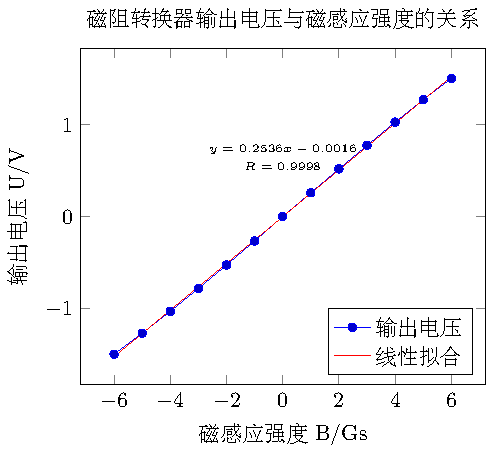
\includegraphics[width=\linewidth]{a}
      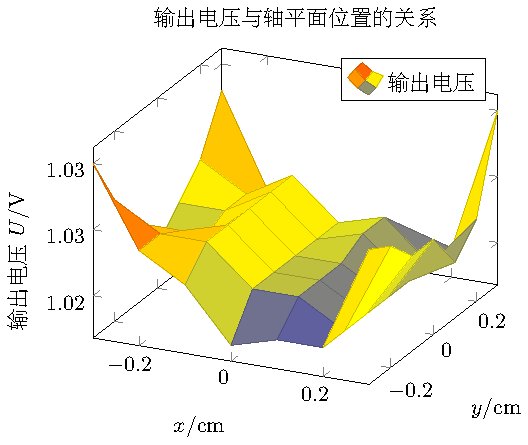
\includegraphics[width=\linewidth]{b}
    \end{column}
    \begin{column}{0.50\textwidth}
      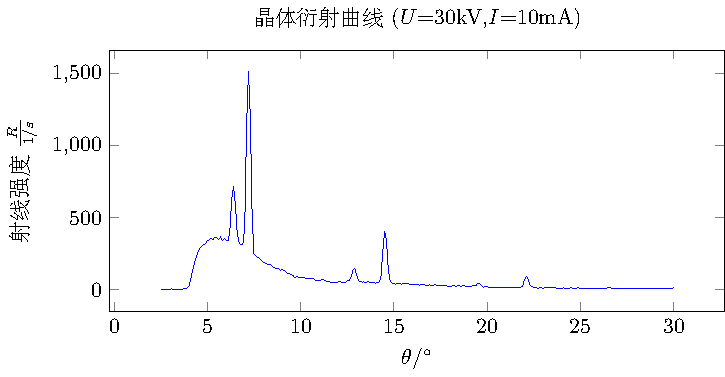
\includegraphics[width=\linewidth]{c}
      \begin{columns}
        \begin{column}{0.5\linewidth}
          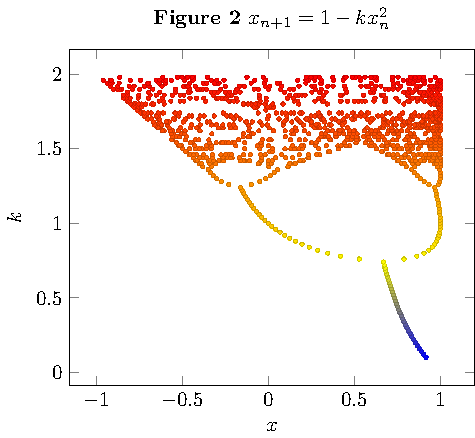
\includegraphics[width=\linewidth]{d}
        \end{column}
        \begin{column}{0.5\linewidth}
          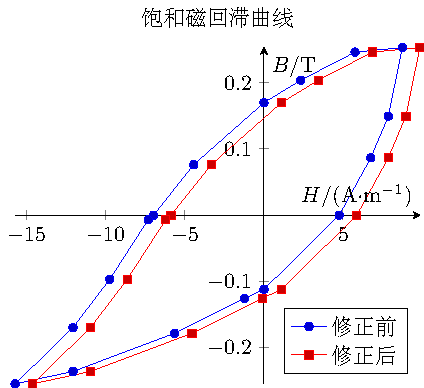
\includegraphics[width=\linewidth]{e}
        \end{column}
      \end{columns}
    \end{column}
    \begin{column}{0.25\textwidth}
      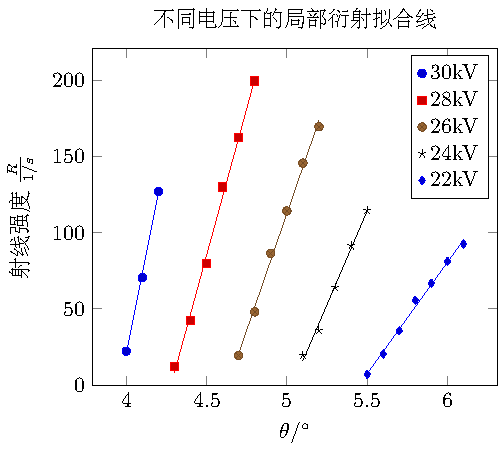
\includegraphics[width=\linewidth]{f}
      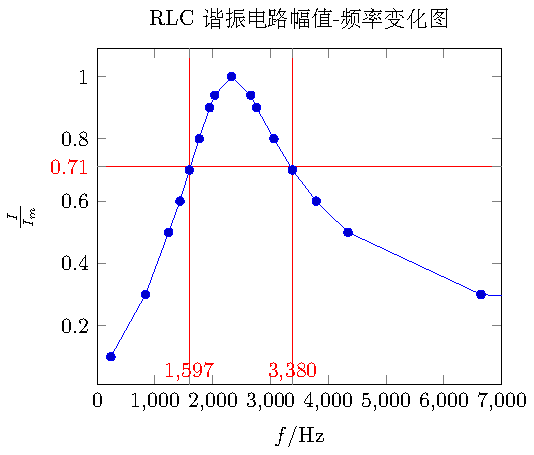
\includegraphics[width=\linewidth]{g}
    \end{column}
  \end{columns}
\end{frame}